%! TEX root = ../../supernova_2023.tex
\documentclass[../../super_nova_2023]{subfiles}

\begin{document}
\chapter{今日の星空を描画したい}
\rightline{M1 忠地涼汰}

\piasec{恒星の描画}
前回のSuper Nova\cite{a}では任意の時刻・位置から見える星空を計算した。
具体的には赤道座標系から地平座標系への変換を行った。
今回は地平座標系から二次元平面への変換を行い、実際に星空を描画してみよう。
等距離射影の全天周画像を作成する。
任意の天体の地平座標系における方向余弦$(x,y,z)^\top$を画像上の座標$(u,v)^\top$
へ次式で変換する。
\vspace{-3mm}
\begin{align}
	\begin{pmatrix}
		u \\ v \\
	\end{pmatrix}
	=
	\frac{1-\frac{2}{\pi} \sin^{-1}{z}}{\sqrt{x^2 + y^2}}
	\begin{pmatrix}
		x \\ y \\
	\end{pmatrix}
	\notag
\end{align}

恒星を描画する時に恒星の明るさによって円の大きさを変化させると見やすい。
5等級小さくなると明るさは100倍になり、
明るさと描画面積が比例すると考えれば、
恒星の視等級を$m$、0等星の描画半径を$r_0$とすると
描画半径は$r = r_0 \lambda^m$となる。
ここで、理論的には$\lambda = \sqrt[10]{\frac{1}{100}} \approx 0.63$であるが、
実際には$\lambda = 0.7$程度が見やすい。
\begin{tcolorbox}
	\scriptsize
	$\lambda$とは・・・星の明るさと描画半径を結びつけるために導入したパラメータのようなもの\par
	$r = r_0 \lambda^m$ とおいて明るさ$A(m)$を面積で $ A(m) = \pi r^2 = \pi r_0^2 \lambda^{2m} $と表す. 
	5等大きくなると明るさ(面積)が$\frac{1}{100}$倍なので
	\[\frac{A(m+5)}{A(m)} = \frac{\pi r_0^2 \lambda^{2m+10}}{\pi r_0^2 \lambda^{2m}} = \frac{1}{100} \Leftrightarrow \lambda^{10} = \frac{1}{100} \Leftrightarrow \lambda = ^{10}\sqrt{\frac{1}{100}} \]
\end{tcolorbox}



\piasec{2023年3月12日20時に調布市で見える星空}
ヒッパルコス星表などから恒星の赤経赤緯を参照し、
2023年3月12日20時に調布市から見える星空を計算して描画する。
今回はヒッパルコス星表の約12万個の恒星と星座線・星座名・天の川データ\cite{b}をPythonで描画してみた。
南の空にシリウスが見えますね。%\mylove
\begin{figure}[h]
	\centering 
	\leavevmode
	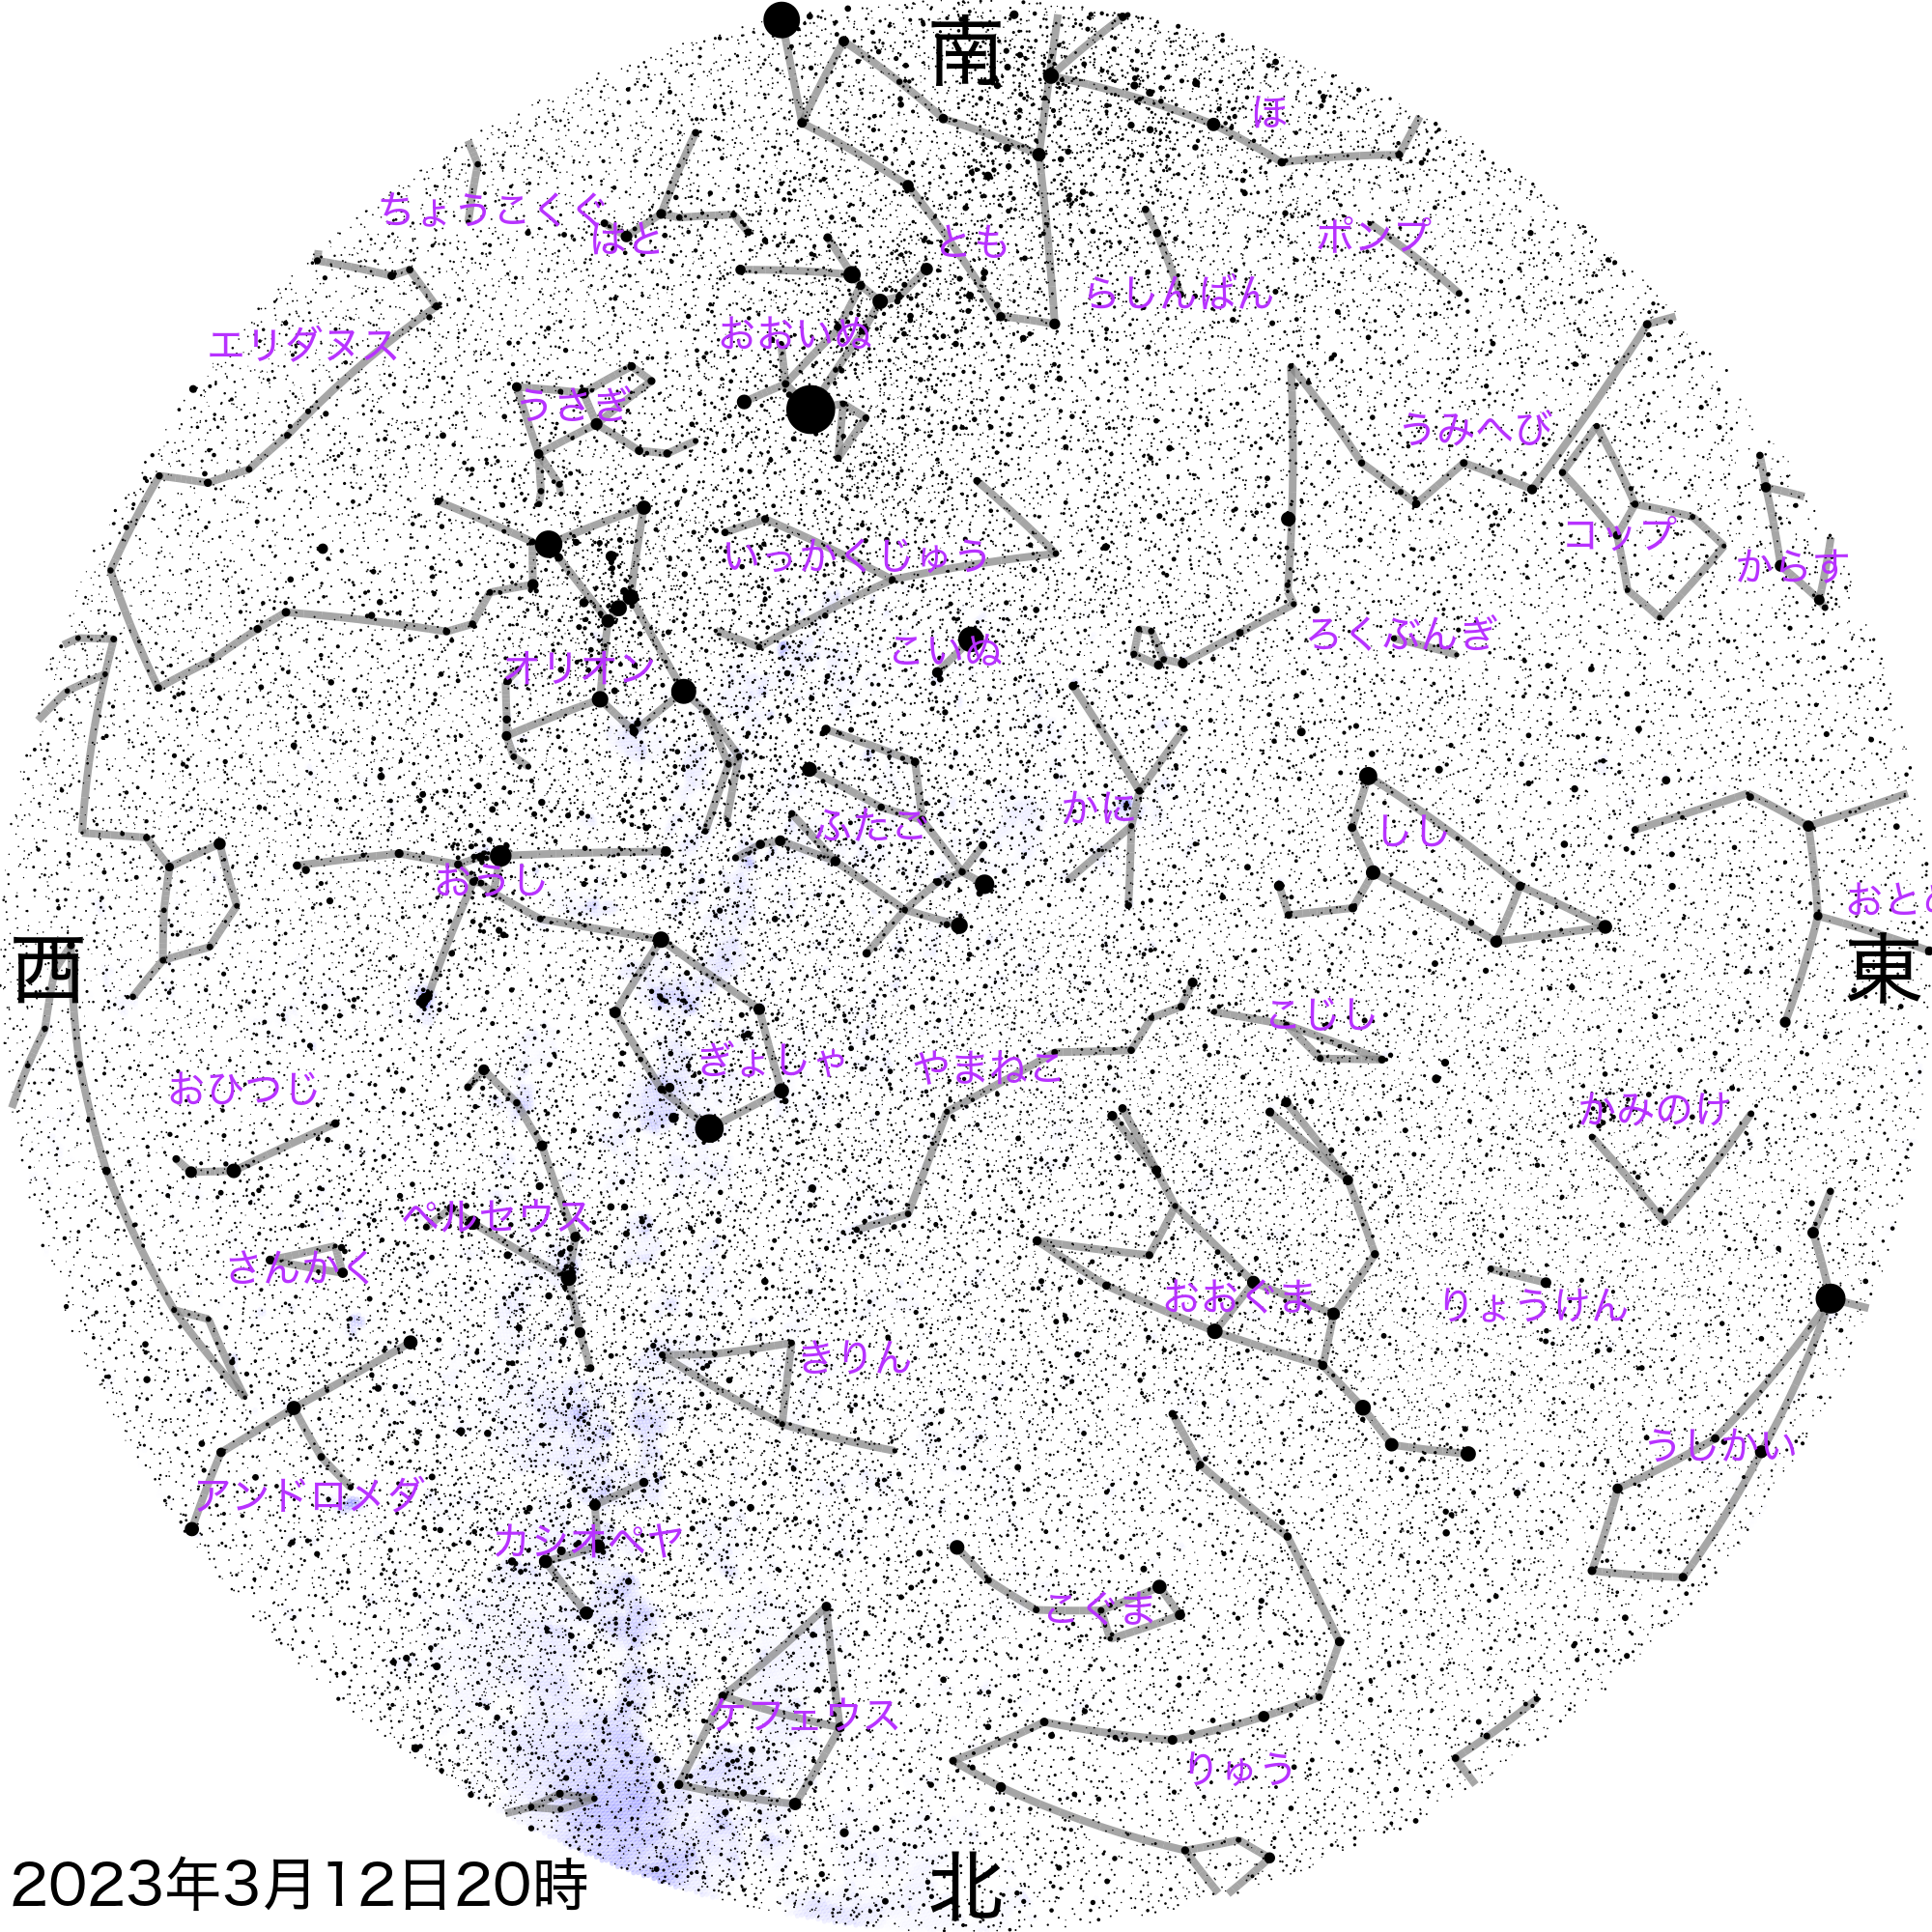
\includegraphics[width=0.55\textwidth]{figures/Tadachi/piari.png}
\end{figure}

\vspace{-3mm}
\begin{thebibliography}{1}
	\bibitem{a} 電気通信大学天文部, Super Nova 2022 調布祭特別号, \url{http://www.astro.club.uec.ac.jp} .
	\bibitem{b} Astro Commons, \url{http://astro.starfree.jp/commons}.
\end{thebibliography}
\end{document}
